\subsection{sLDS model learns states that correspond to distinguishable behaviors}
\label{sec:slds:3.2.3}
An alternative approach to address jitter in the joint positions would be to use a method that directly incorporates observation noise into the model and can thus learn learn smoothed representations of the observations. The model would then use the smoothed representations to infer the discrete states, thereby avoiding the problem where flickering in the keypoints is absorbed into the model as a state transition. Switching linear dynamical systems (SLDS) models provide a principled way to do precisely that by extending the AR-HMM framework to include an additional layer in between the observations and discrete states (Fig. ). This layer consists of a set of continuous latents that are governed by a Gaussian noise term ($\mathcal{N}(0,Q)$ in Fig. ), thus acting as a denoised version of the lower-level observations. We write the continuous state update as, 

\begin{equation} \label{eq:slds_3}
x_t = A_{z_t} x_{t-1} + \epsilon \qquad \epsilon \sim \mathcal{N}(0,Q)
\end{equation}
where $x_t$ is the vector of continuous latent states at the current time point, $x_{t-1}$ is the vector of latents at the previous time point, $A$ is a model-inferred dynamics matrix governing how the latents evolve over time in the current discrete state $z_t$, and $\epsilon$ is additive Gaussian noise with covariance $Q$. Note the similarity in structure between Eq. \ref{eq:slds_3} and Eq. \ref{eq:slds_1} in Section \ref{sec:slds:3.2.2}. To connect the continuous latents to the observations we have, 

\begin{equation} \label{eq:slds_4}
y_t = C_{z_t}x_{t} 
\end{equation}
where $y_t$ is the vector of observations at the current time point and $C$ is a model-inferred loading matrix governing the mapping between the continuous latents and observations for the discrete state at the current time point. If the number of continuous latents $p$ is set to be equal to the number of observations $q$, than $C$ will be square and is often enforced to be the identity matrix $I$, thus directly equating each latent to a smoothed version of each observation. However, this setting is not required; even in the case where $C$ is square it does not have to be the identity, and when $p<q$ the continuous latents then serve as a smoothed, lower-dimensional representation of the observations (akin in some ways to performing dimensionality reduction on the observations themselves). As for the discrete state updates, they follow the same formula as the AR-HMM (see Eq. \ref{eq:slds_2}). 

\begin{figure}[t!]
  \begin{center}
    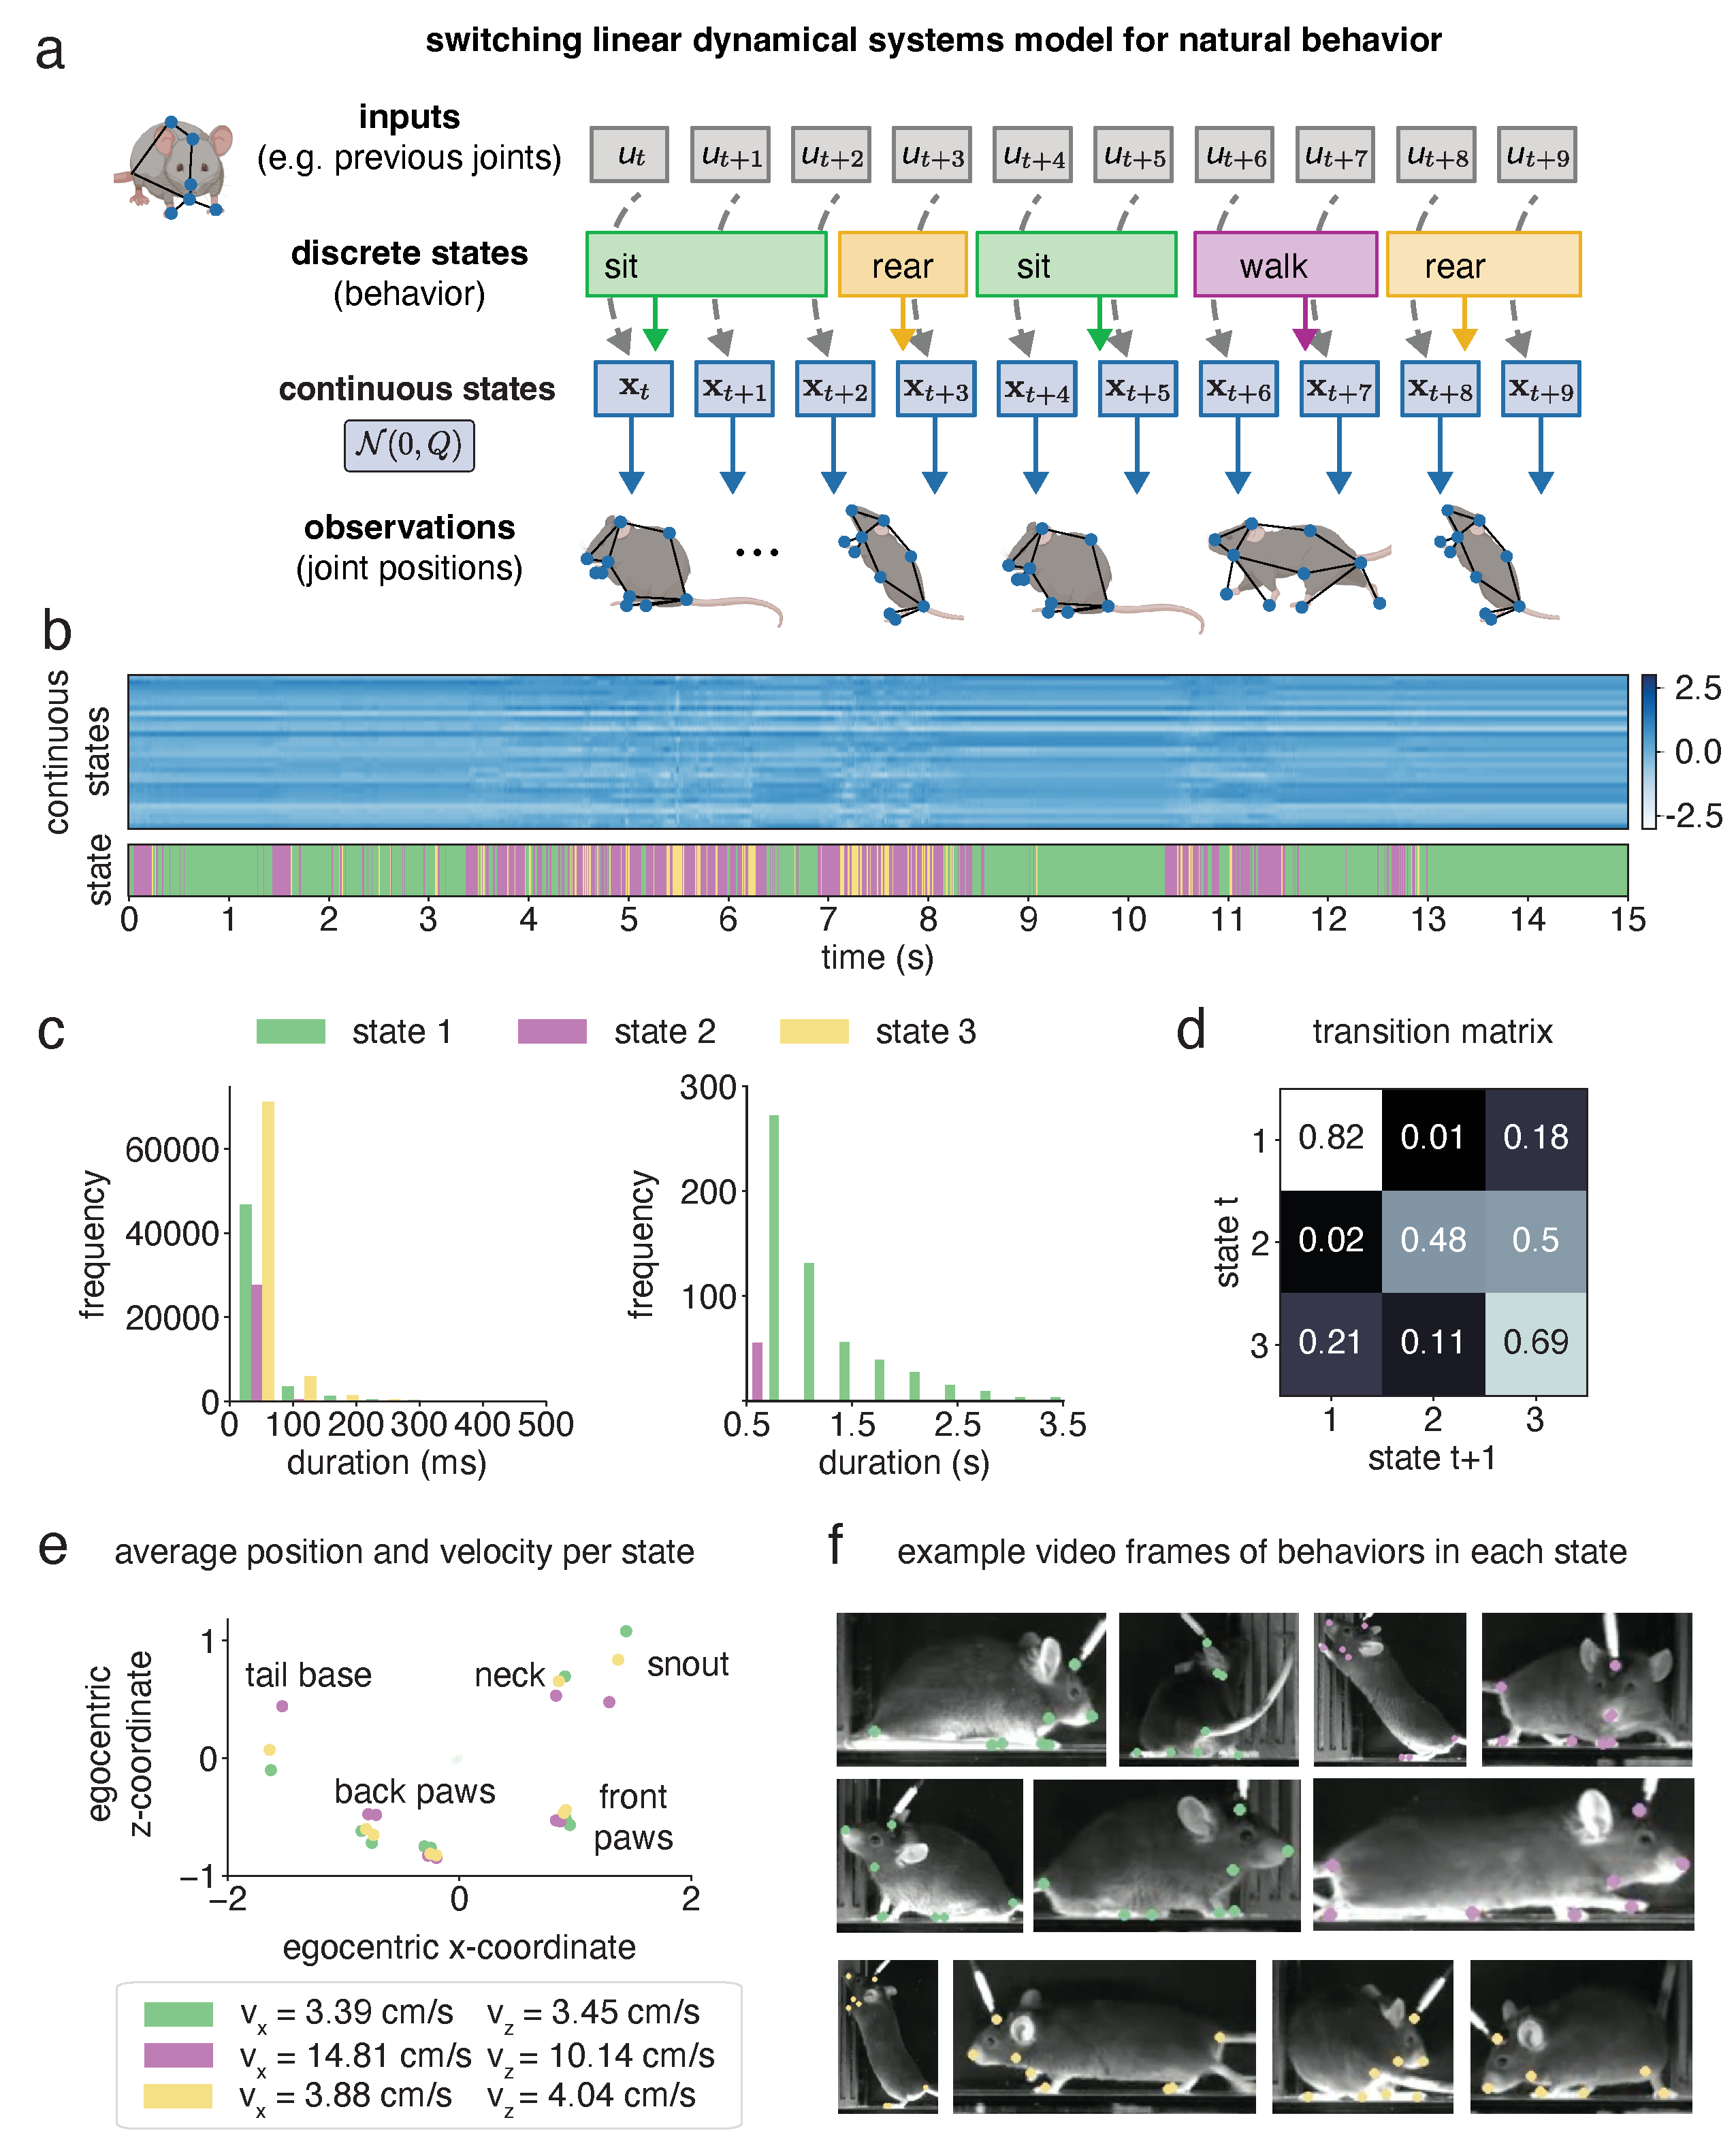
\includegraphics[width=0.90\linewidth]{ch3-slds/slds-figures/Fig3.pdf}
    \caption[SLDS inferred states are longer than AR-HMM inferred states and are more distinguishable in the behaviors they represent]{\textbf{SLDS inferred states are longer than AR-HMM inferred states and are more distinguishable in the behaviors they represent.} (a) SLDS schematic. The model follows the same general structure as the AR-HMM except there is an additional layer of continuous latent states between the discrete states and the observations. (b) Inferred continuous latents (top) with the SLDS inferred most-likely state of the animal at each time point (bottom) for a 15-second time window. (c) Histograms of the state durations for instances of discrete states that last less than 0.5 seconds (left) and greater than 0.5 seconds (right). (d) Discrete state transition probabilities. }
    \label{fig:slds:3}
  \end{center}
  \vspace{-0.5cm}
\end{figure}
\begin{figure}[t!]
  \contcaption{ (e) Average x- and z-positions (length and height view of mouse) of each joint in each state (top) along with per-state average velocities (bottom). (f) Screen grabs of examples of the animals' pose positions in frames the SLDS assigned to each state.}% Continued caption
\end{figure}

We fit a 3-state SLDS to the data with $q=p$ but without requiring $C=I$. Visual inspection of the inferred continuous latents reveals how they act as smoothed representations of the observations, with fewer discontinuities and sudden jumps (Fig. 3b, top, compare to Fig. 2b). The inferred discrete state sequences... 
